\documentclass[12pt]{article}
\usepackage[a4paper]{geometry}
\usepackage[utf8]{inputenc}
\usepackage{fancyhdr}
\usepackage{lastpage}
\usepackage{graphicx, wrapfig, subcaption, setspace, booktabs}
\usepackage{graphicx}
\usepackage[T1]{fontenc}
\usepackage[font=small, labelfont=bf]{caption}
\usepackage[protrusion=true, expansion=true]{microtype}
\usepackage[english]{babel}
\usepackage{sectsty}
\usepackage{url, lipsum}
\usepackage[T1]{fontenc}
\usepackage{icomma}
\usepackage{siunitx}
\usepackage{ragged2e}
\usepackage{amsmath}
\usepackage{comment}
\usepackage{enumerate}
\usepackage{anysize}


\newcommand{\HRule}[1]{\rule{\linewidth}{#1}}
\onehalfspacing
\setcounter{tocdepth}{5}
\setcounter{secnumdepth}{5}

\begin{document}

\begin{titlepage}

\title{ \normalsize 
        \begin{center}
        
\includegraphics[height=6cm]{logo.png}
        \end{center}
        \LARGE \textsc{\textbf{Universidad De Sonora}} \\ \bigskip
		\Large División de Ciencias Exactas y Naturales \\
        Licenciatura en Física \\ \bigskip
        \bigskip
        Física Computacional I
		\\ [0.1cm]  
		\HRule{2pt} \\
		\Large \textbf{{Evaluación 2}} \\
        \textit{\textbf{"El Atractor de Lorenz, ejemplo de Caos dinámico"}}
		\HRule{2pt} \\
		\normalsize \vspace*{0.001\baselineskip}}
        
\date{\bigskip \Large Hermosillo, Sonora  \hspace*{\fill}  26 de Abril de 2018}

        
\author{
		\Large\textbf{ Michelle Contreras Cossio} \\ \bigskip
        \\ \bigskip
       \Large Profr. Carlos Lizárraga Celaya}
       \end{titlepage}
       \maketitle
       

\newpage
\pagestyle{plain}

\section{Introducción}
El Sistema de Lorenz es un sistema de ecuaciones diferenciales ordinarias, que tiene su nombre por el primero que lo estudio, Edward Lorenz, este tiene la particularidad que ciertos parámetros pueden llevar a soluciones caóticas, formando un atractor llamado de igual manera, "Atractor de Lorenz".\\

Lorenz descubrió el caos por accidente, cuando quería hacer un modelo matemático de la convección atmosférica, usando las siguientes ecuaciones diferenciales:

\begin{equation}
\frac{dx}{dt}=\sigma (y-x)
\end{equation}
\begin{equation}
\frac{dy}{dt}= x(\rho -z)-y
\end{equation}
\begin{equation}
\frac{dz}{dt}=xy -\beta z
\end{equation}

El siguiente artículo utiliza código de Geoff Boeing para animación y visualización del atractor de Lorenz, para realizar la evaluación 2, se realizaron 3 ejemplos donde con diferentes condiciones iniciales. 

\section{Resultados del análisis (Gráficas)}

Se muestran las gráficas que se crearon. NOTA: los gifs se encuentran en el github.

\clearpage

\begin{itemize}
\item \textbf{Ejemplo \#1:} 

Con valores: sigma = 10, beta = 8/3 y rho = 28 

\begin{itemize}
\item \underline{Gráficas de visualización:} 

\begin{center}
        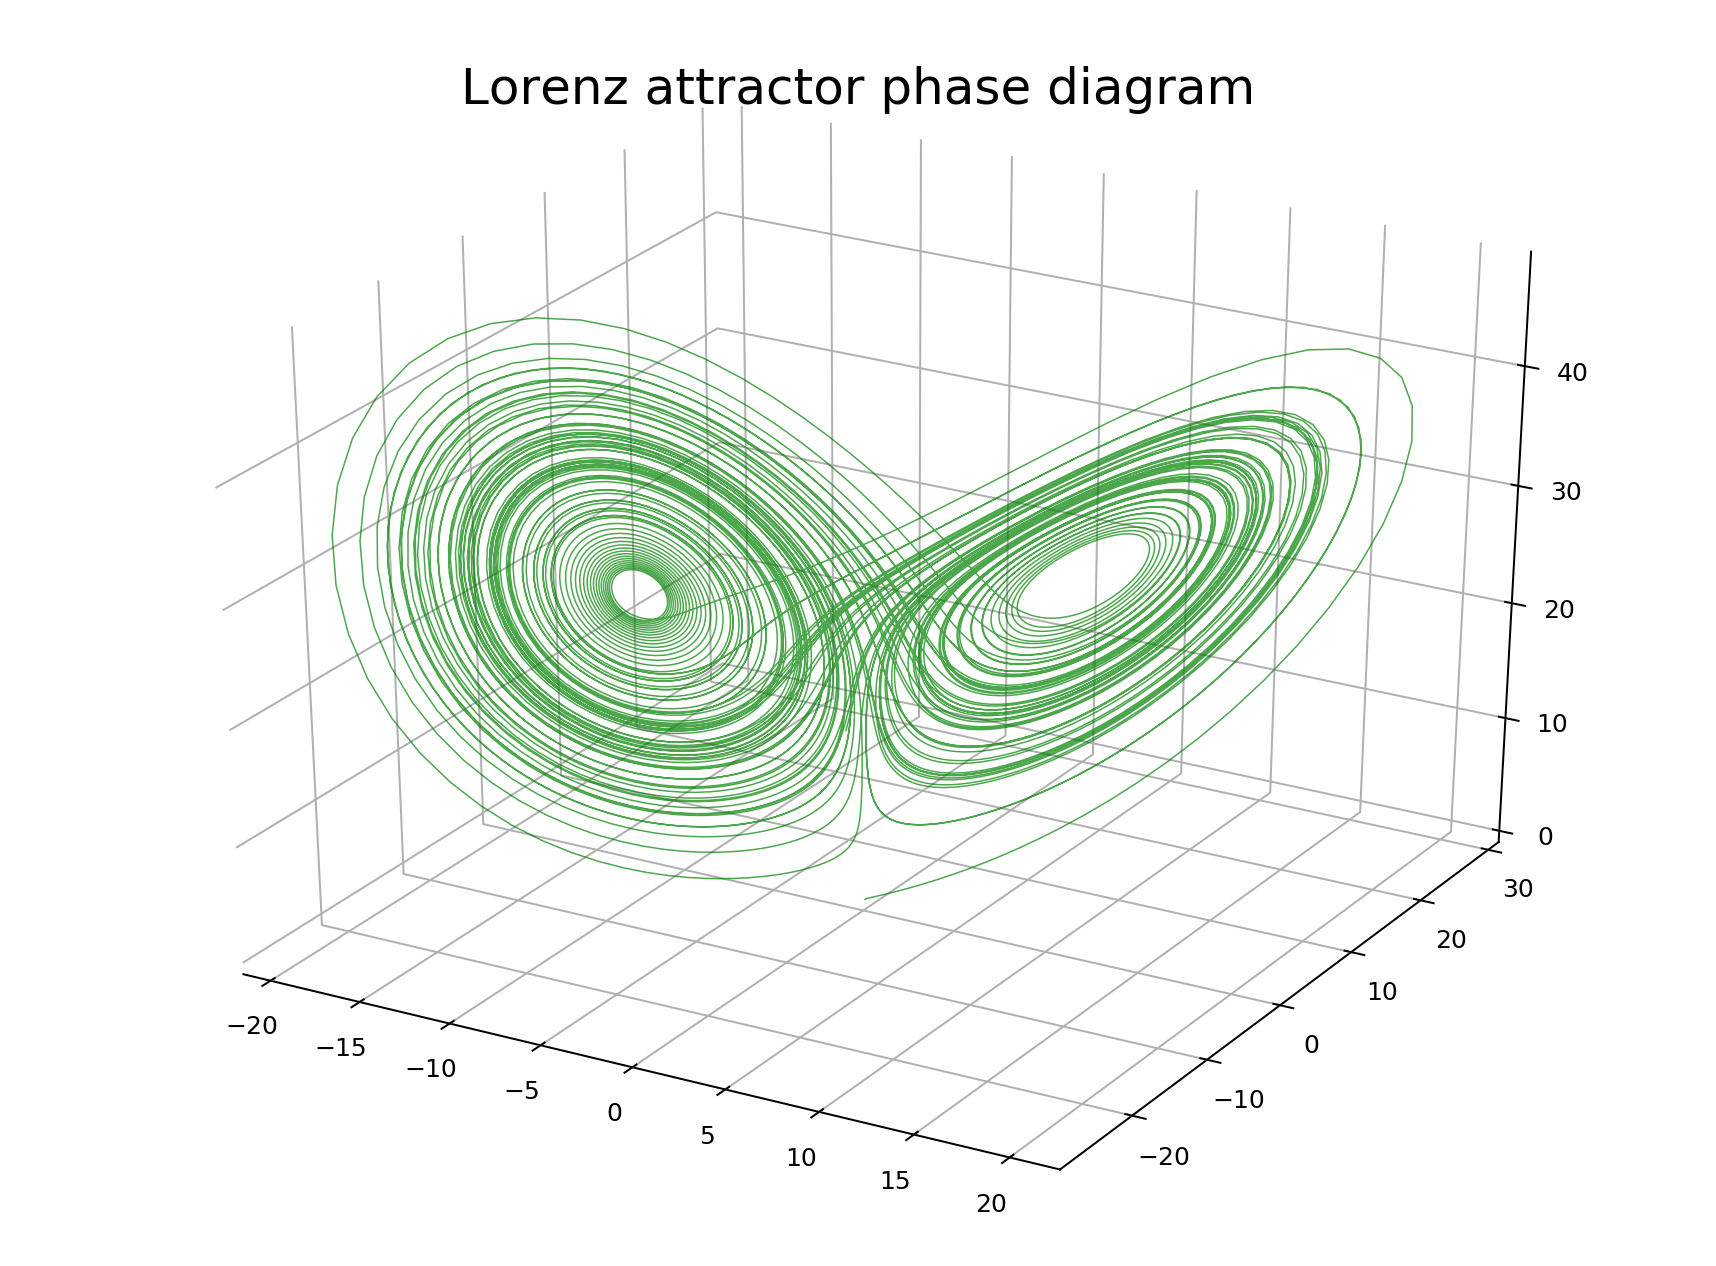
\includegraphics[height=10cm]{lorenz-attractor-3d-1.png}
\end{center}

Esta gráfica del atractor de Lorenz de 3D muestra el modelo "canónico" donde se visualiza perfectamente el caos, aún cuando las posiciones iniciales no se encuentren tan cerca de los atractores.

\begin{center}
        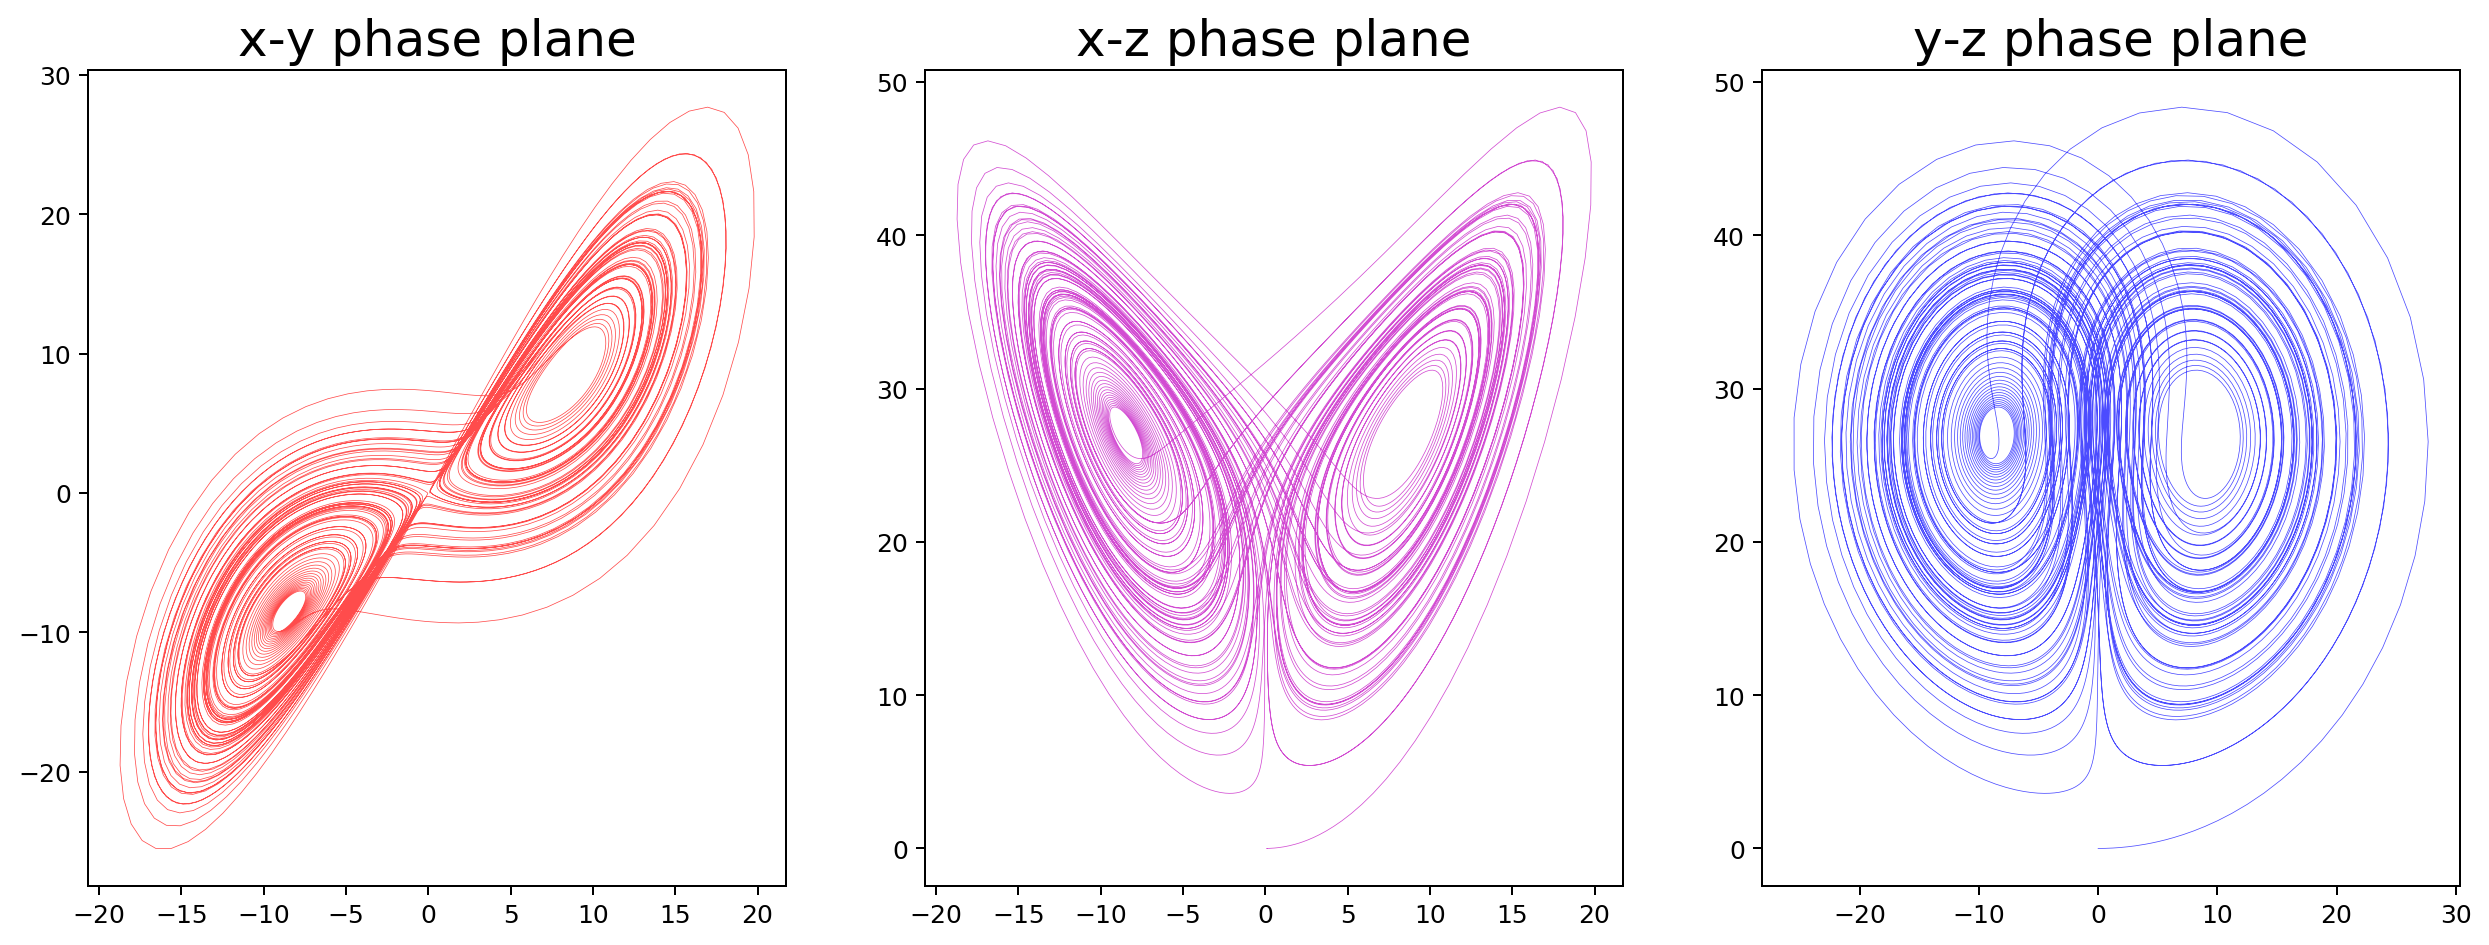
\includegraphics[height=5.5cm]{lorenz-attractor-phase-plane-1.png}
\end{center}

Estos gráficos son bastante útiles porque permiten una mejor visualización de la gráfica en 3D, observando más perspectivas, en la gráfica xz es donde se logra ver la característica "mariposa" de los fenómenos caóticos.

\begin{center}
        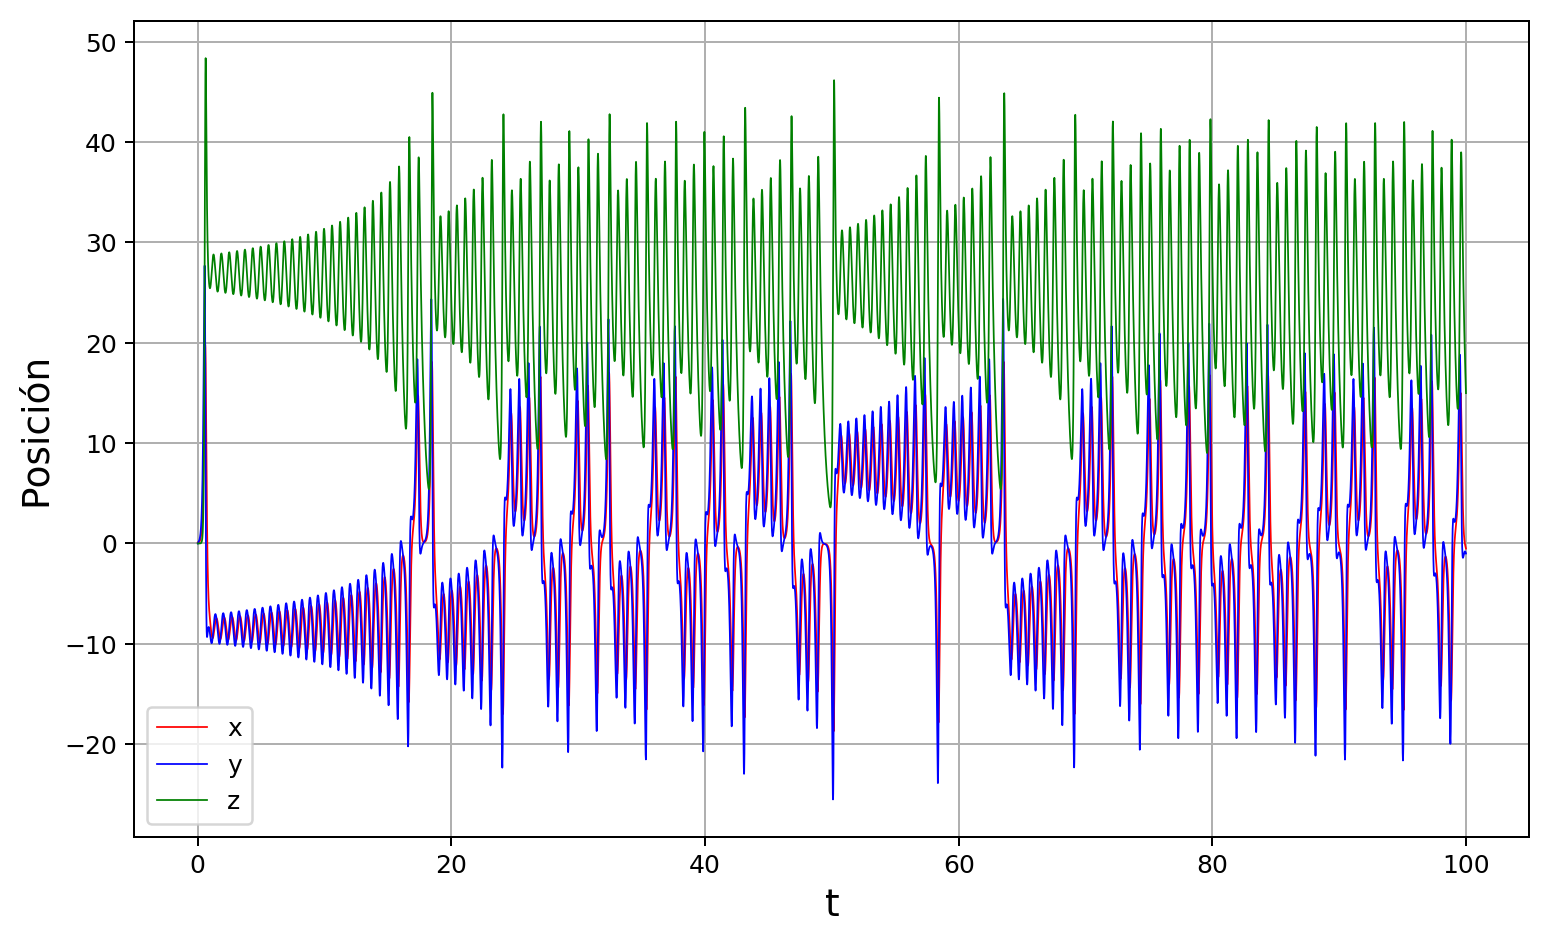
\includegraphics[height=7.5cm]{lorenz-attractor-position-time-1.png}
\end{center}

Por último, para estas condiciones iniciales, podemos ver la gráfica de la posición en x,y,z con respecto al tiempo. Vemos que las posiciones en x,y son similares puestas una sobre otra, mientras que la de z se parece, pero toma valores más altos. 

\end{itemize}

\item \textbf{Ejemplo \#2:} 

Con valores: sigma = 28, beta = 4 y rho = 46.92

\begin{itemize}
\item \underline{Gráficas de visualización:} 

\begin{center}
        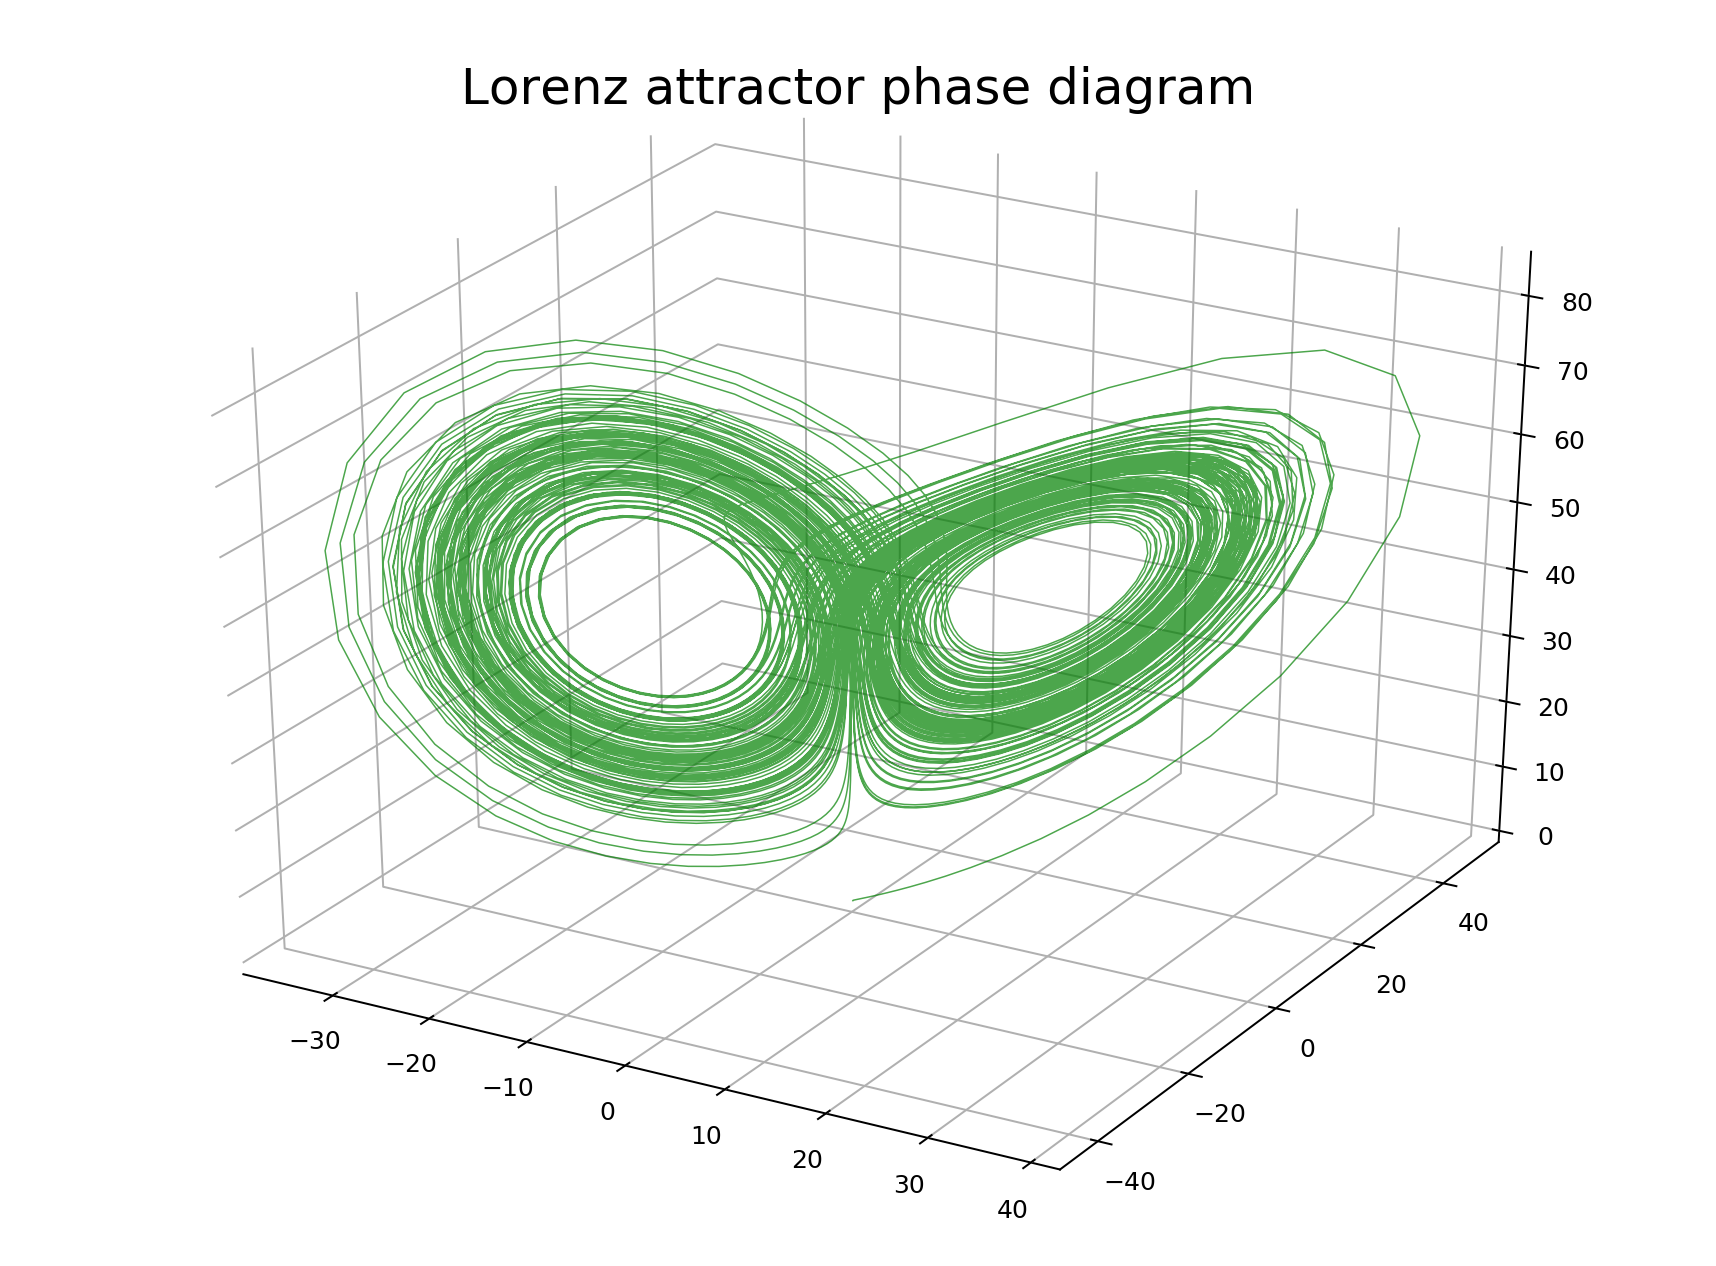
\includegraphics[height=10cm]{lorenz-attractor-3d-2.png}
\end{center}

En este diagrama de 3D, podemos visualizar como el atractor es un poco más grueso, con las mismas condiciones iniciales, además es un poco más grande, pero alrededor del origen.

\begin{center}
        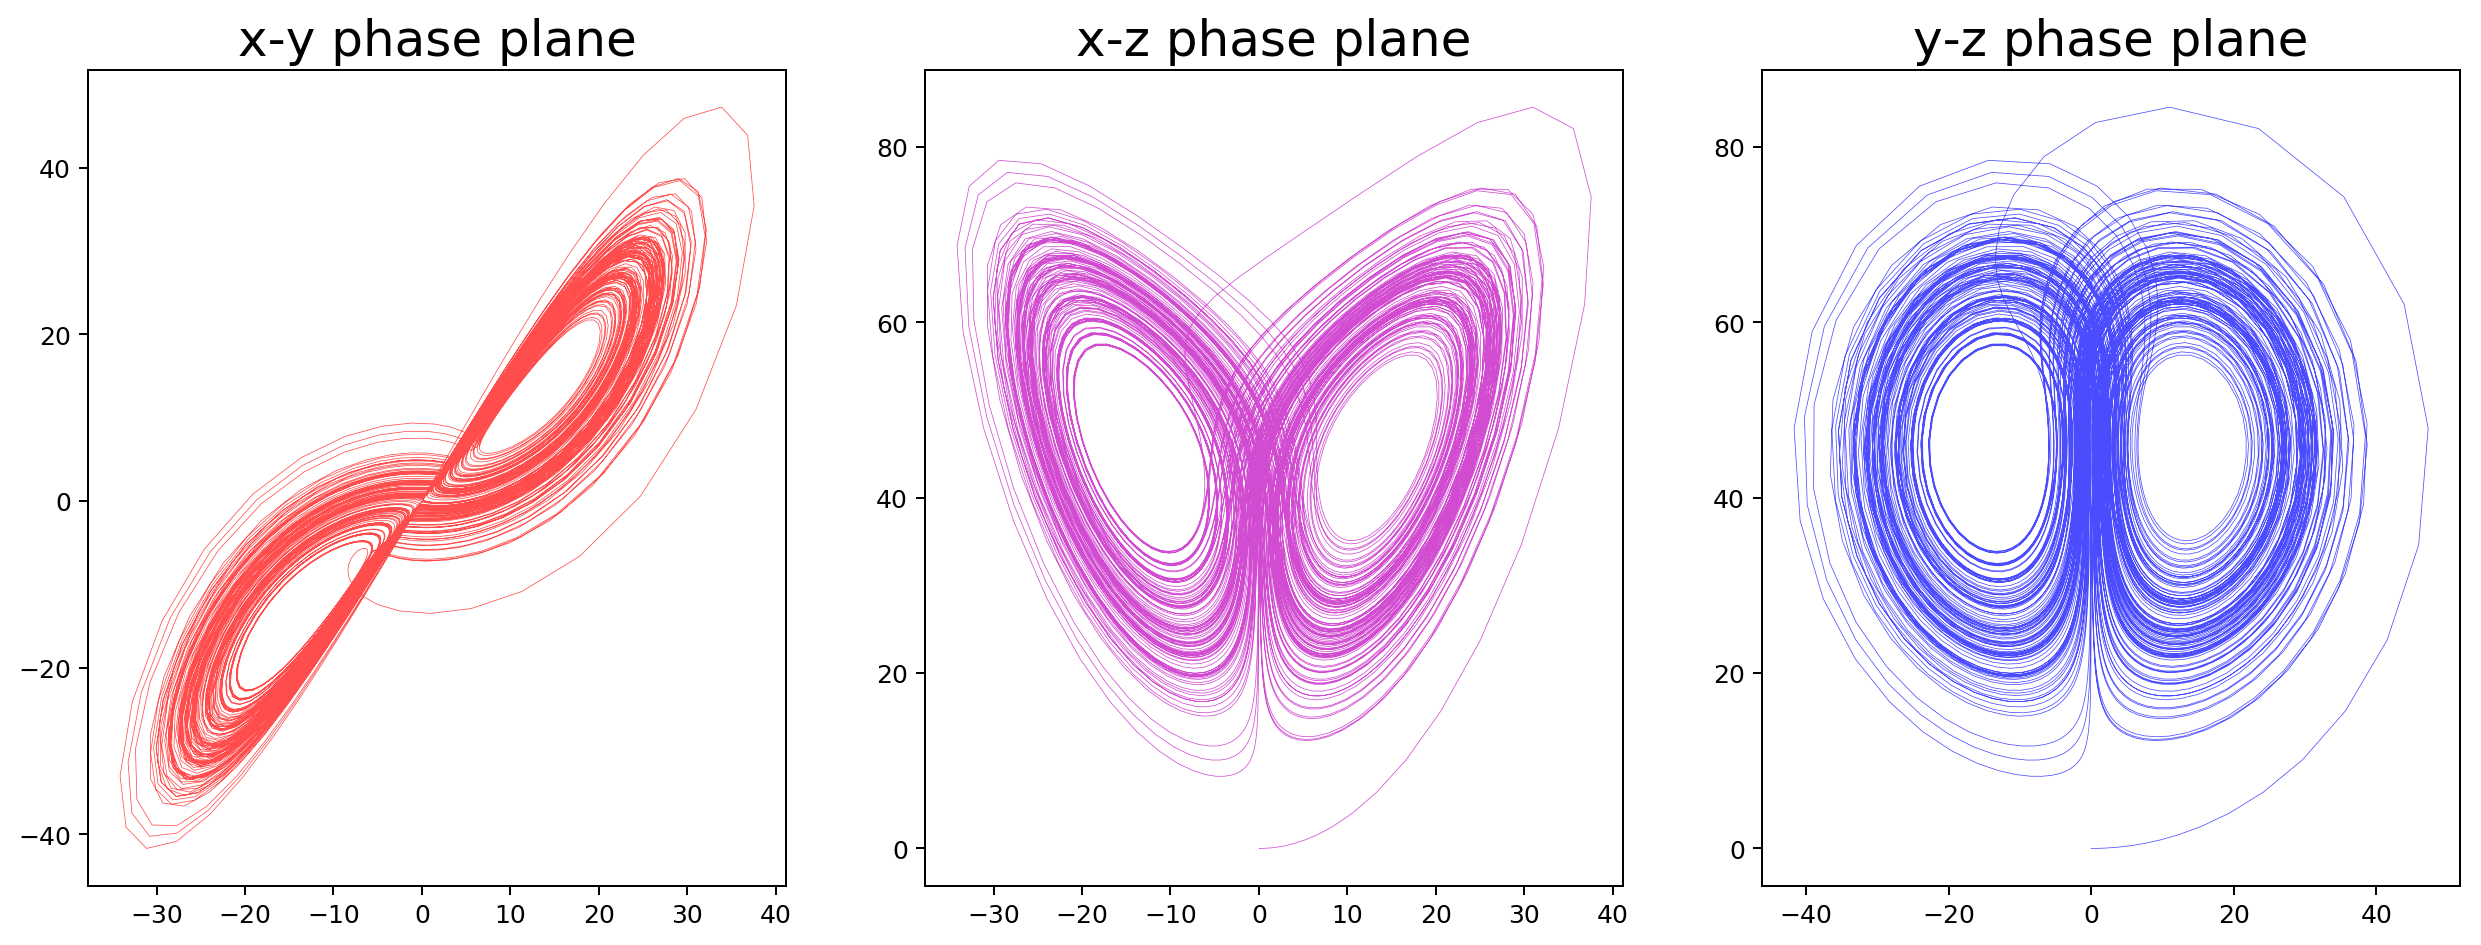
\includegraphics[height=5.5cm]{lorenz-attractor-phase-plane-2.png}
\end{center}

Estos gráficos se parecen bastante a los anteriores, pero de igual manera son más gruesos, con un hoyo más pequeño, también se puede ver la gráfica en forma de mariposa.

\begin{center}
        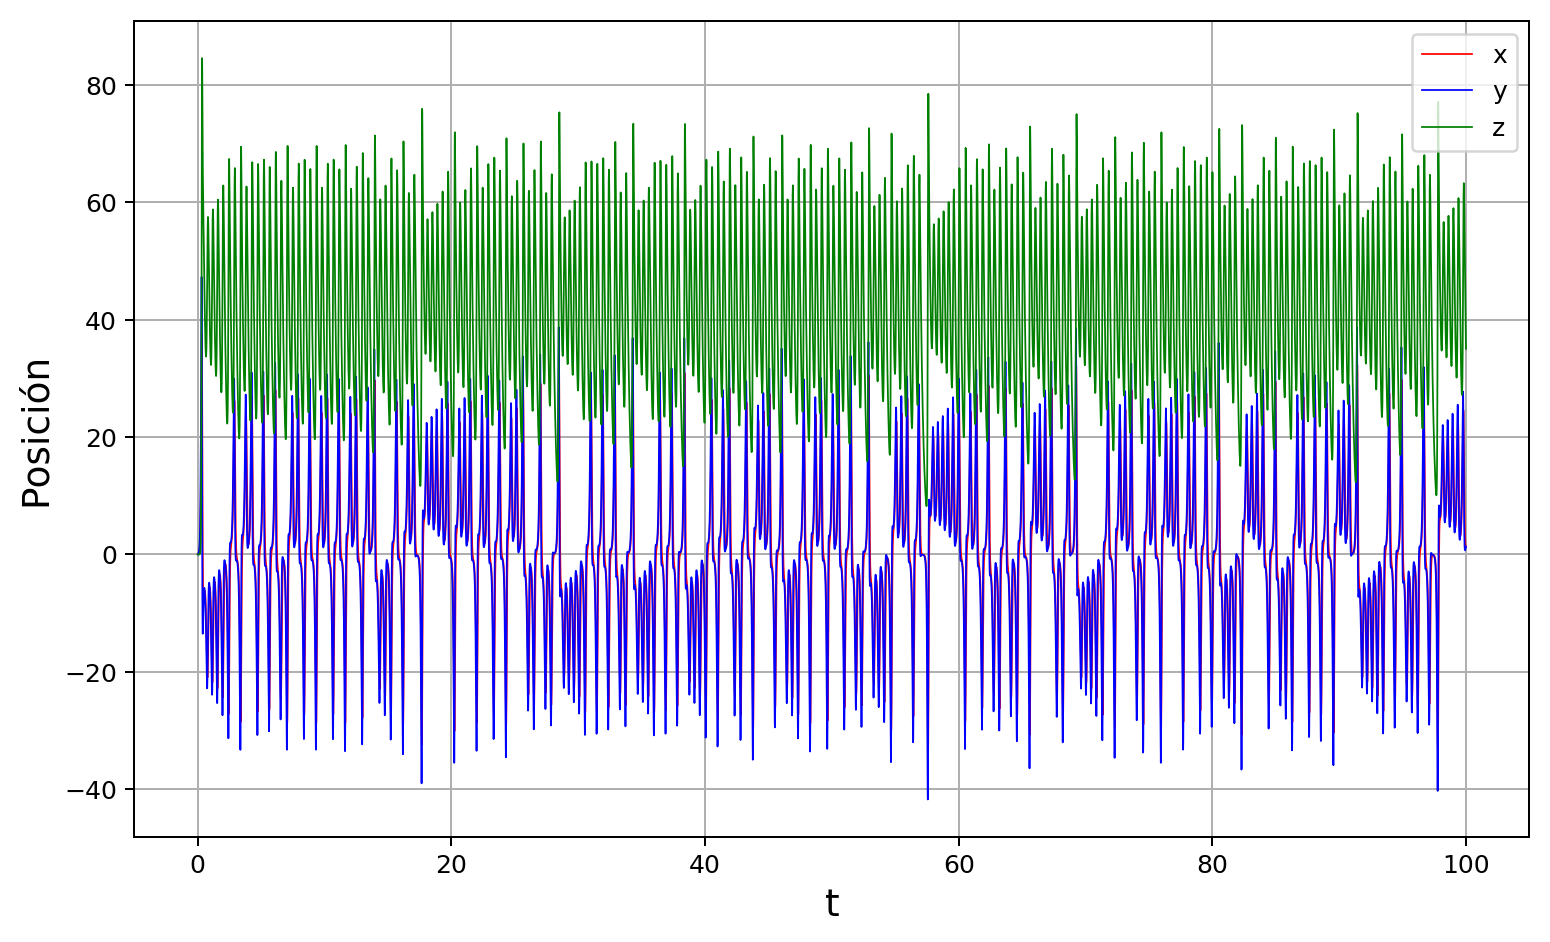
\includegraphics[height=7.5cm]{lorenz-attractor-position-time-2.png}
\end{center}

Está gráfica también es similar al ejemplo anterior, donde las gráficas x,y se parecen mucho y la de z es similar pero más elevada, positiva siempre.

\end{itemize}

\clearpage

\item \textbf{Ejemplo \#3:} 

Con valores: sigma = 10, beta = 8/3 y rho = 99.96.

\begin{itemize}
\item \underline{Gráficas de visualización:} 
\begin{center}
        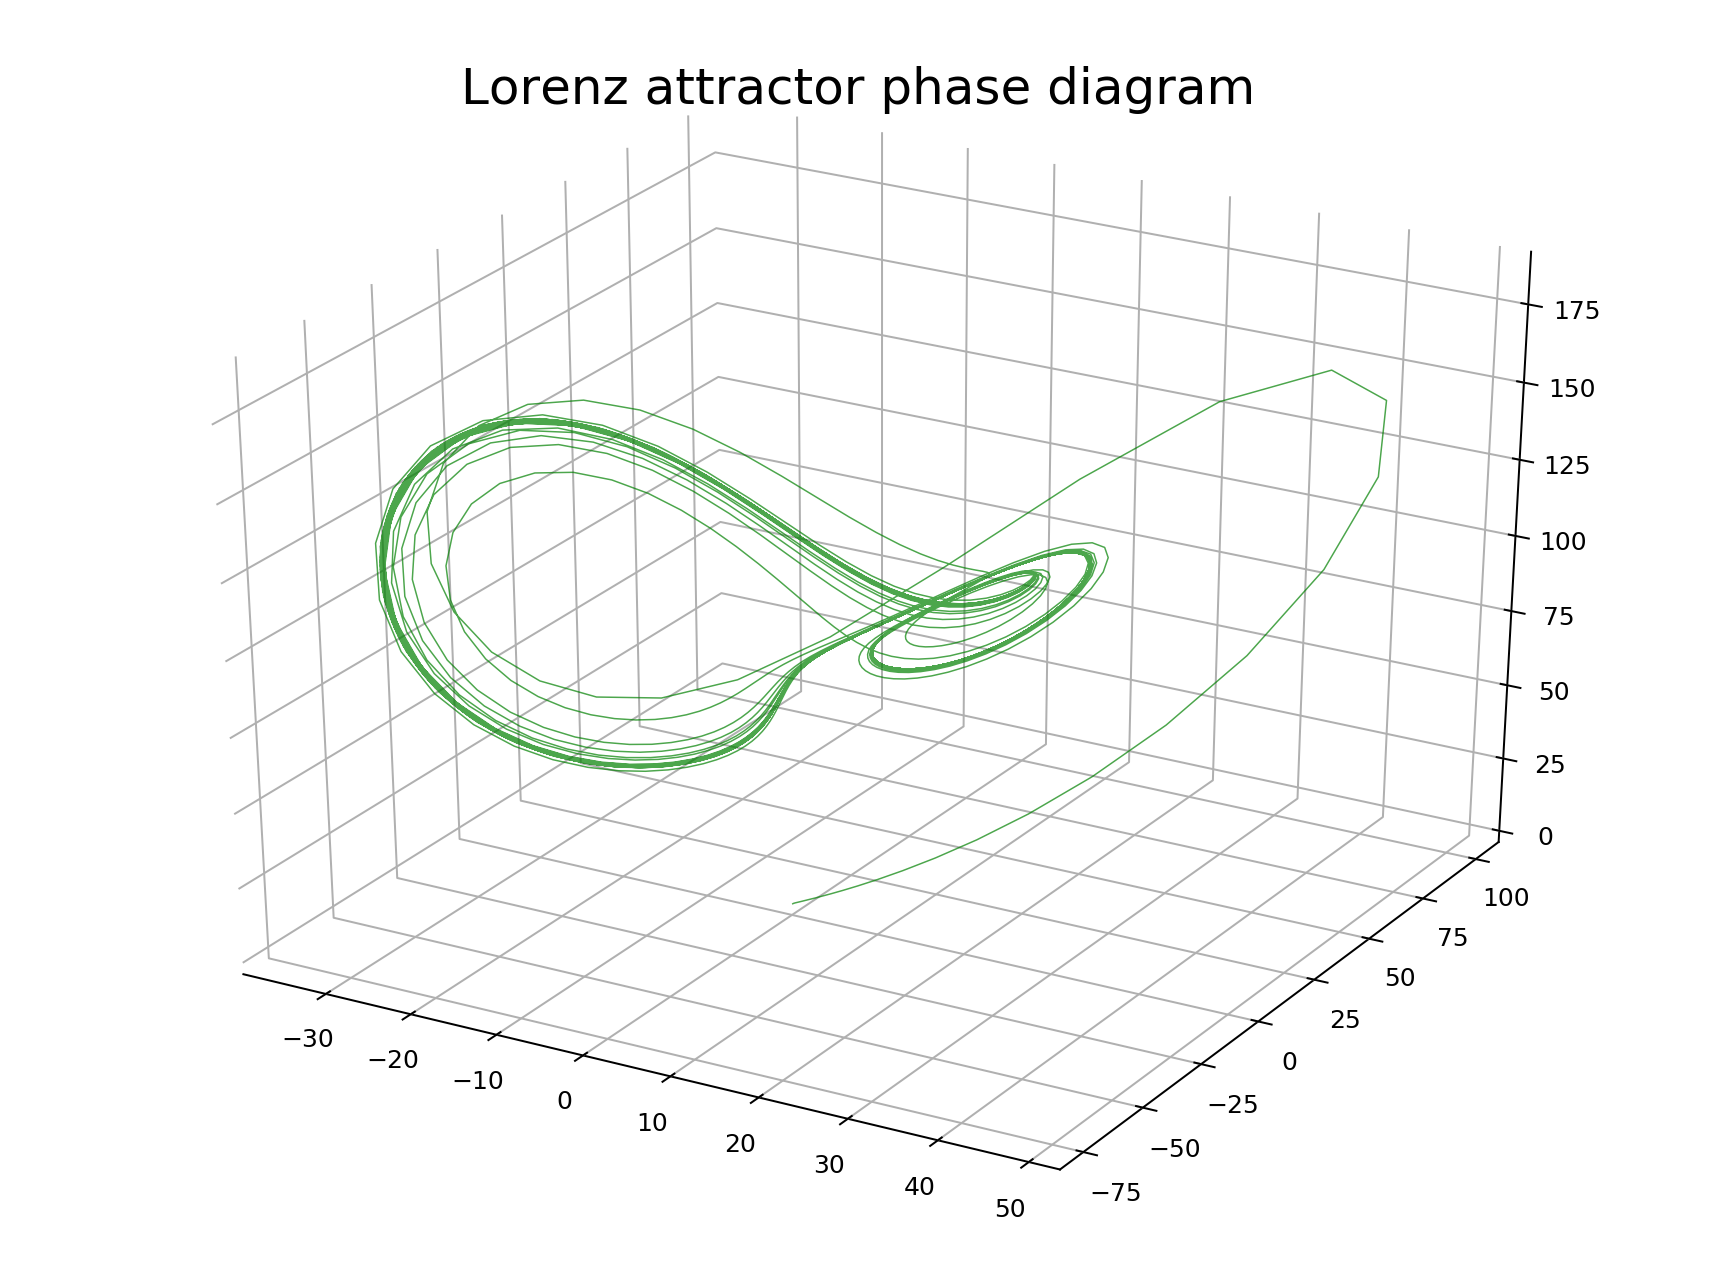
\includegraphics[height=10cm]{lorenz-attractor-3d-3.png}
\end{center}

Por útlimo, este atractor es diferente a los demás, no es tan simétrico, mas recargada al eje x negativo, esto se puede deber al cambio drástico en rho, ya que sigma y beta son iguales que en el ejempo 1. 

\begin{center}
        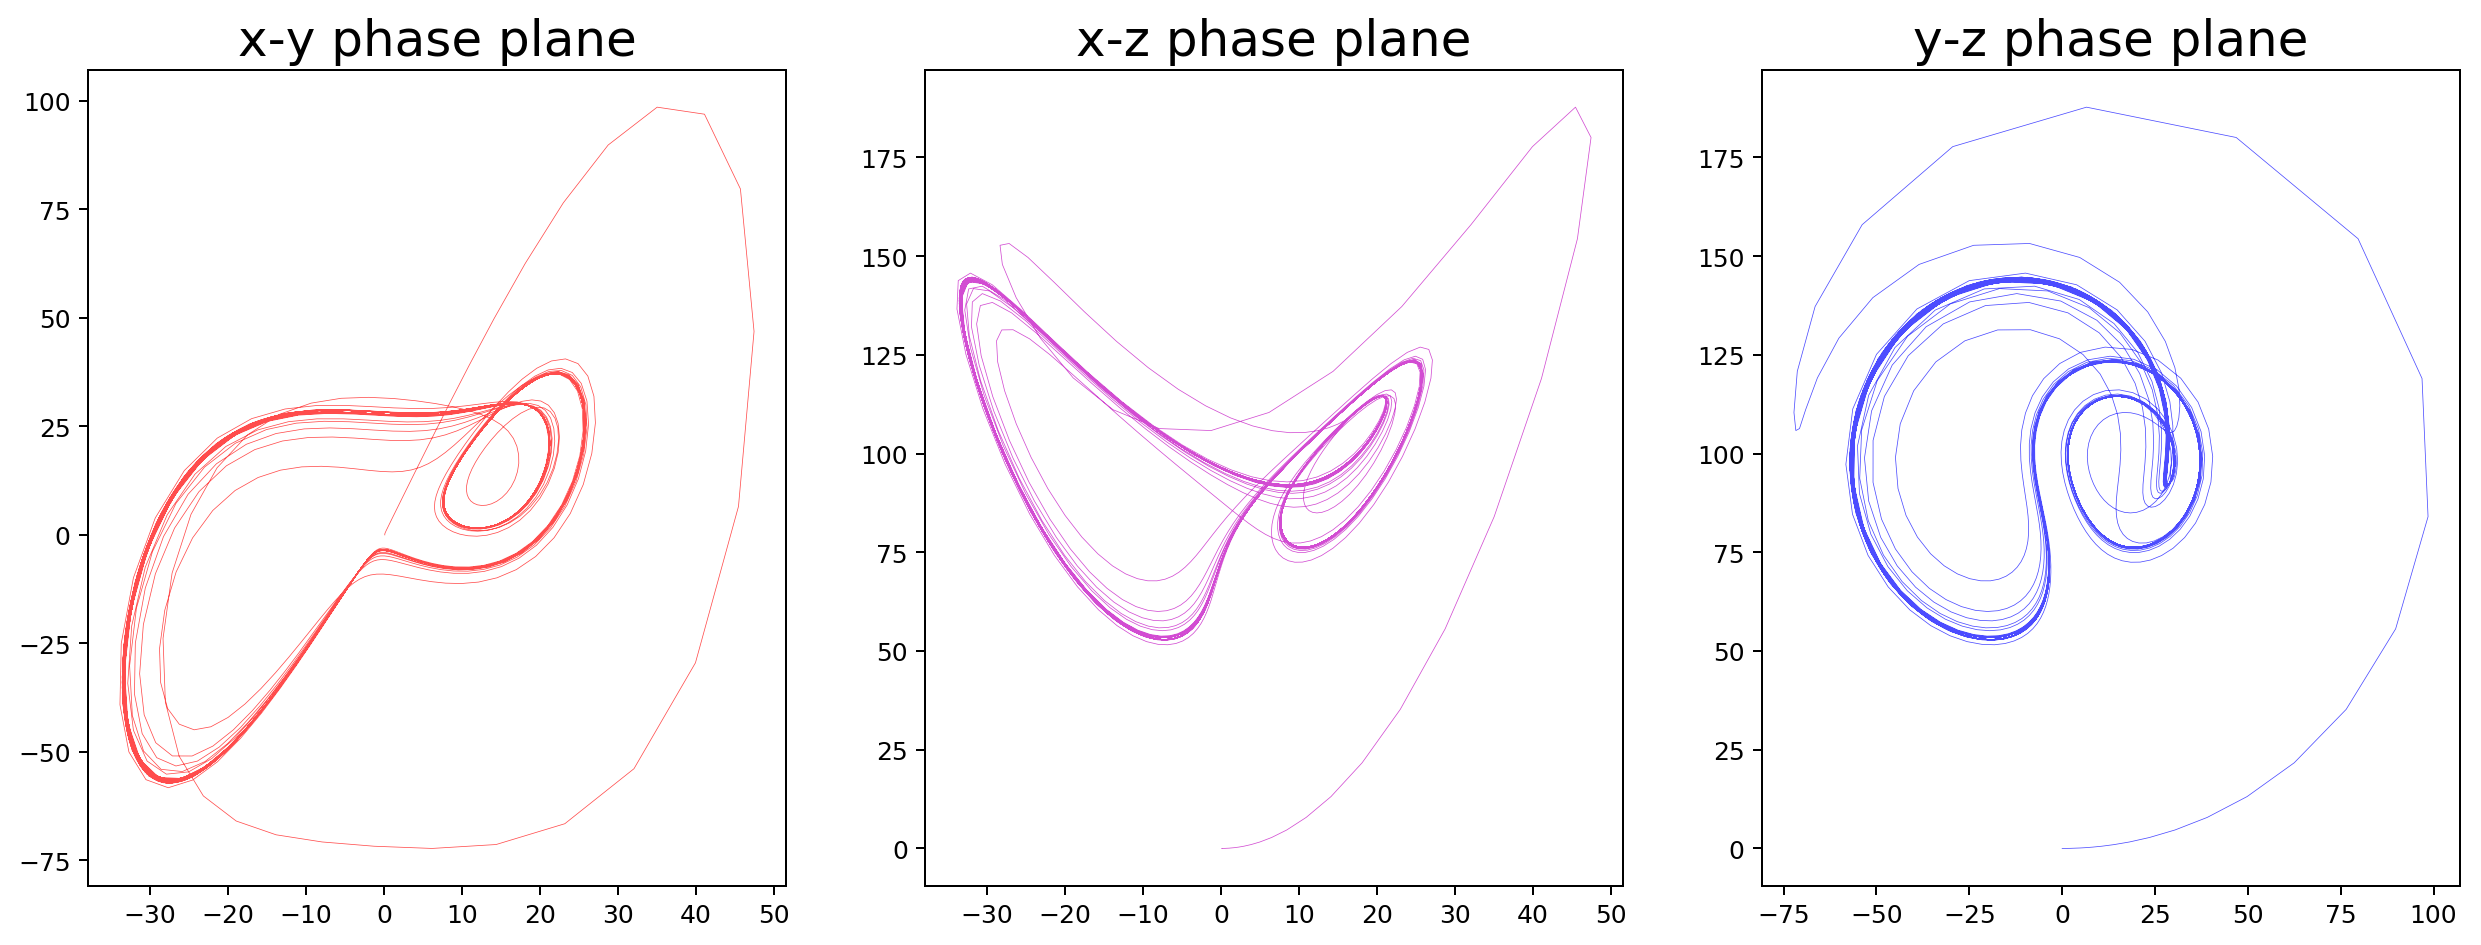
\includegraphics[height=5.5cm]{lorenz-attractor-phase-plane-3.png}
\end{center}

Aquí se ve la diferencia, donde en el plano xz no se muestra la mariposa, se nota la falta de simetría, debido a la condición inicial de posición, empieza el ciclo similar a los demás pero recae en el "ala" izquierda.

\begin{center}
        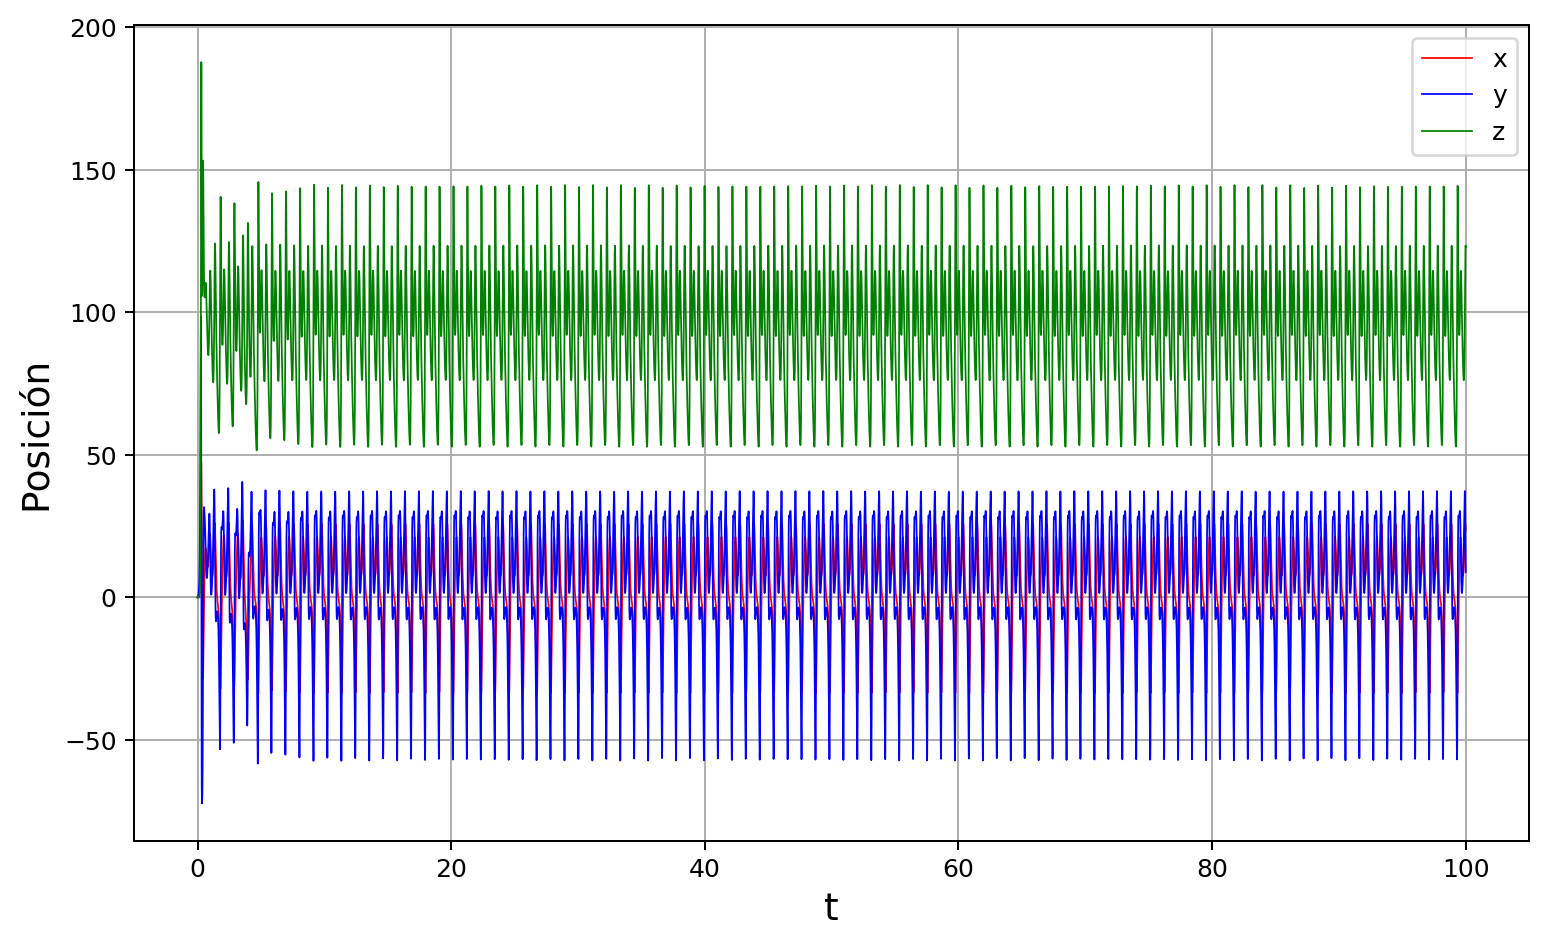
\includegraphics[height=7.5cm]{lorenz-attractor-position-time-3.png}
\end{center}
\end{itemize}

Finalmente, podemos ver que x,y están alrededor del origen, de igual manera se encuentran una sobre la otra, pero en este caso se pueden ver un poco menos solapadas. Mientras que el eje z es positivo siempre, como en las demás. 

\end{itemize}

\clearpage

\section{Conclusiones}

Primero puedo concluir que es bastante interesante observar este tipo de fenómenos que llevan a soluciones caóticas, aunque no sabemos prácticamente nada de esto, me parece algo que quisiera saber a futuro, ya que estos fenómenos se pueden presentar en casos simples y sin avisar.  \\ 

Esta evaluación me gustó, fue fácil de desarrollar, pero a la vez tenía su chiste. 

\section{Bibliografía}
\begin{itemize}
\item Lorenz System (2018). Consultado: 26 de Abril del 2018, de Wikipedia. Sitio web: https://en.wikipedia.org/wiki/Lorenz\_system
\item Animating the Lorenz Attractor with Python (2016). Geoff Boeing. Consultado: 26 de Abril del 2018, de geoffboeing. Sitio web:  http://geoffboeing.com/2016/12/animating-lorenz-attractor-python/
\item Código de Visualización del Atractor de Lorenz (2016). Geoff Boeing. Consultado: 26 de Abril del 2018, de Github. Sitio web:  https://github.com/gboeing/lorenz-system/blob/master/lorenz-system-attractor-visualize.ipynb
\item Código de Animación del Atractor de Lorenz (2016). Geoff Boeing. Consultado: 26 de Abril del 2018, de Github. Sitio web:  https://github.com/gboeing/lorenz-system/blob/master/lorenz-system-attractor-animate.ipynb
\end{itemize}


\end{document}